%v4.4
\subsection{The BigBite Spectrometer}
%
\label{sec:expsetup_bigbite}             
%
Scattered electrons will be detected in the BigBite spectrometer.
The spectrometer consists of a single dipole magnet (with magnetic field approximately 1.2~Tesla-m 
and a detection system, see Fig.~4.  

\begin{figure}[htbp]
\begin{center}
%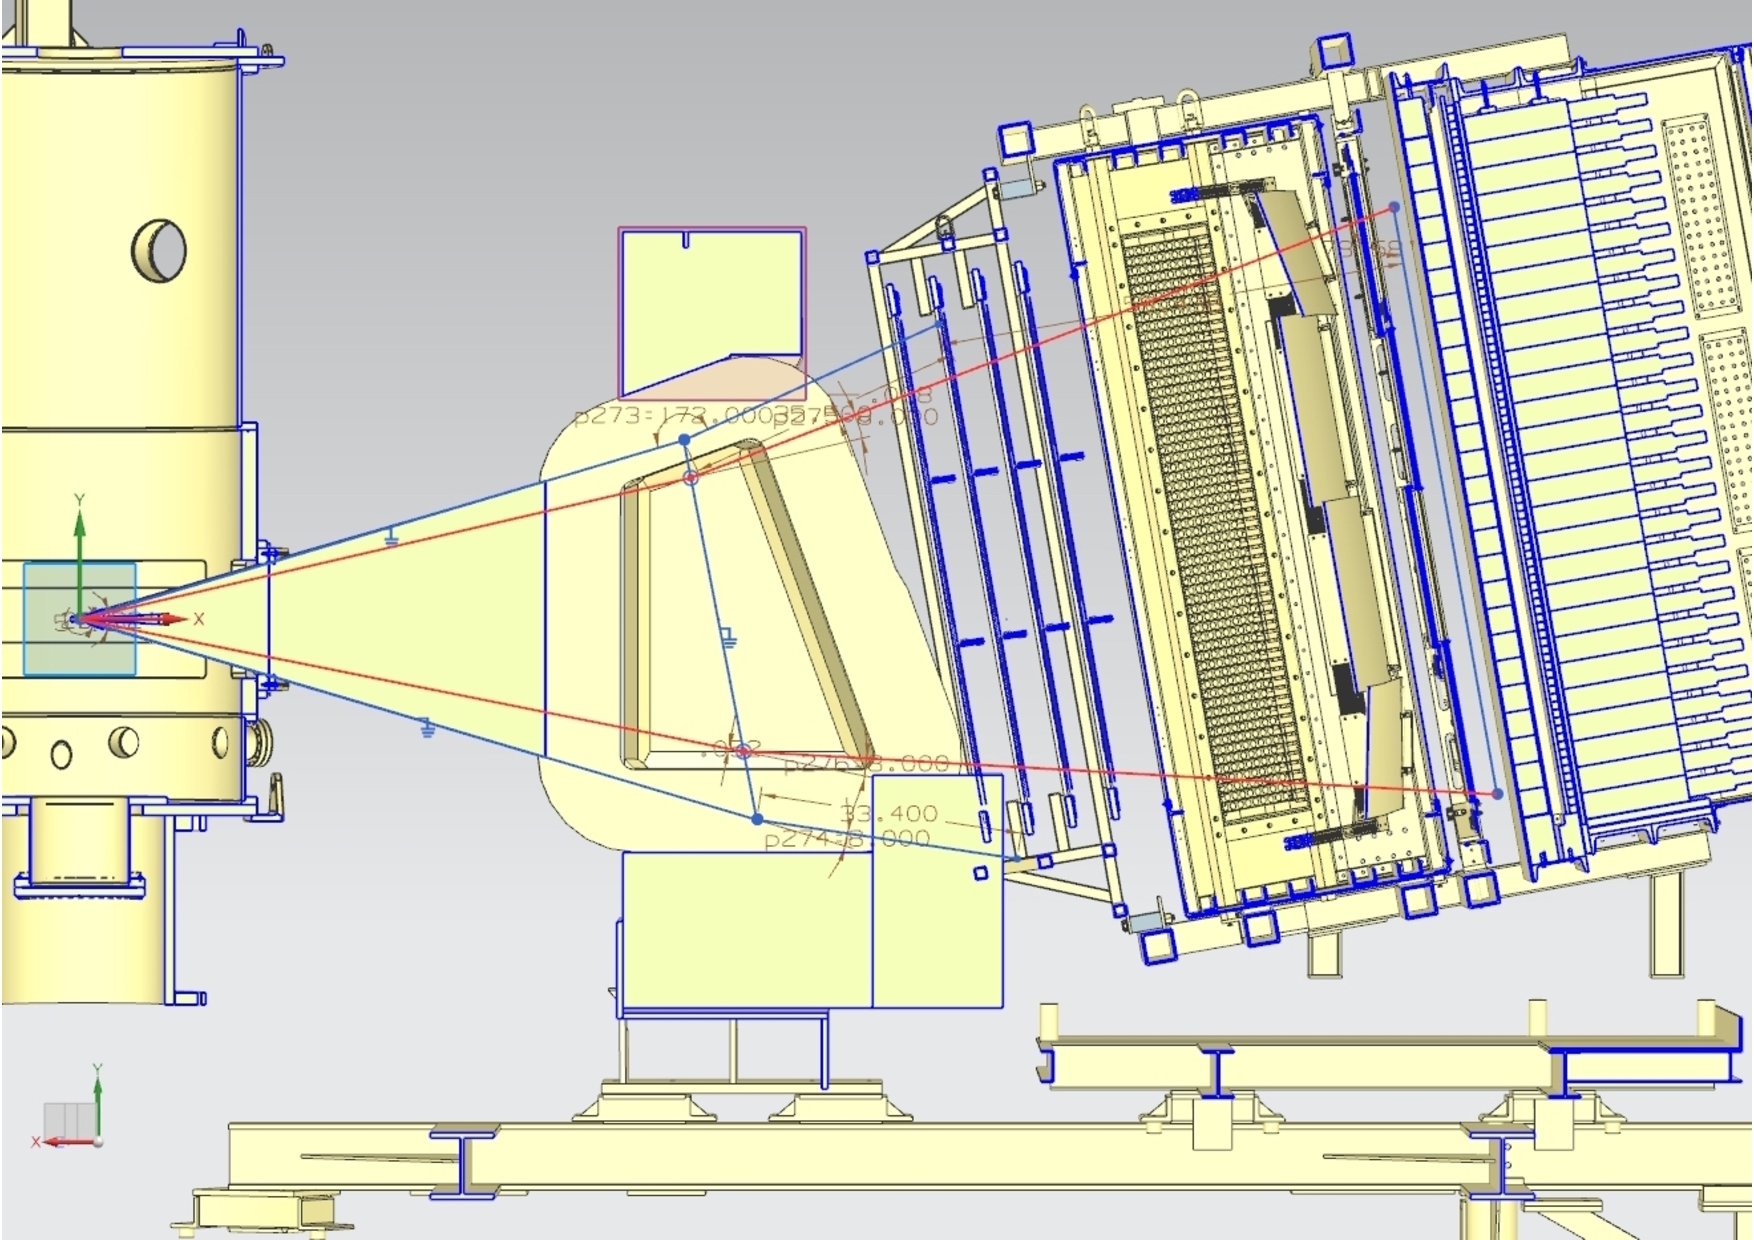
\includegraphics[trim = 5mm 0mm 0mm 0mm, width=0.475\textwidth, angle = 0]{Plots/BB_Side-view.pdf} 
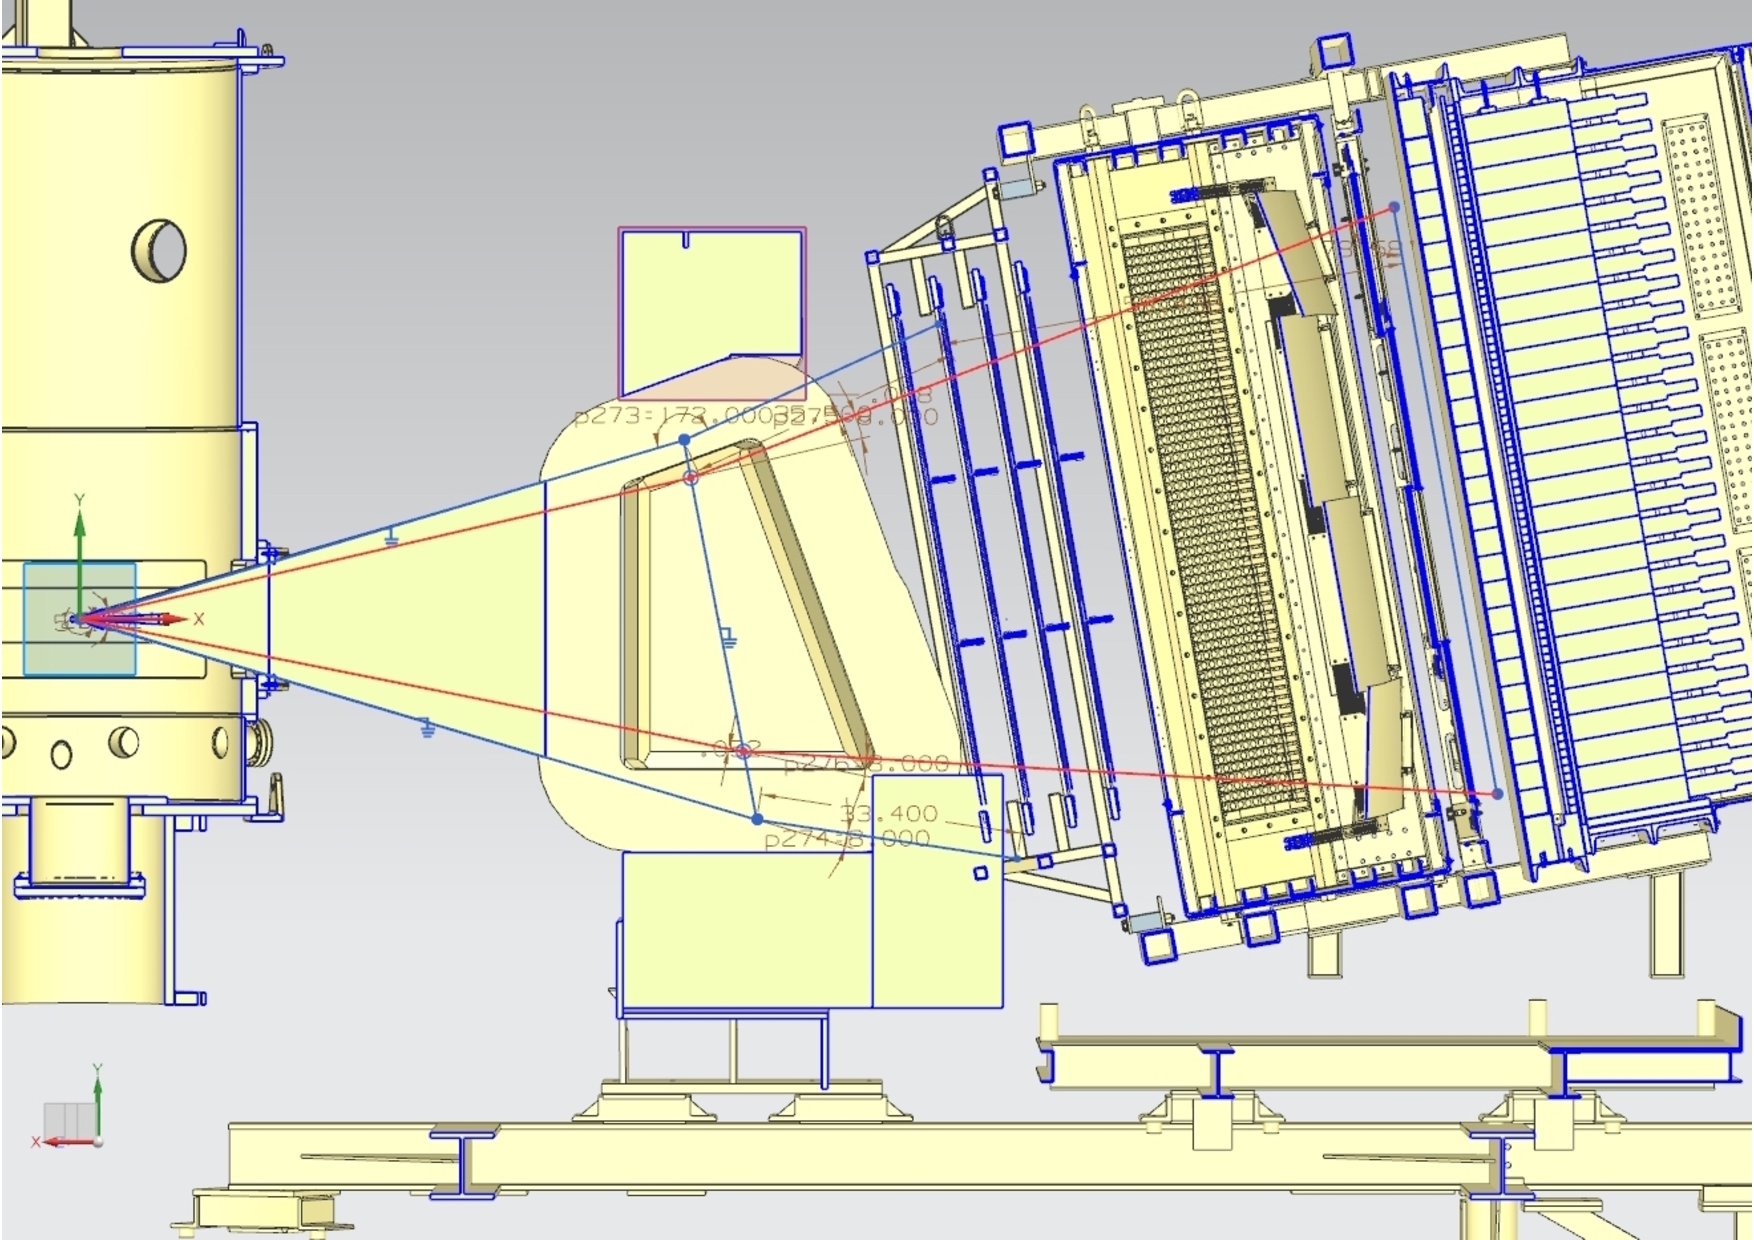
\epsfig{file=Plots/BB_Side-view.pdf, height=3.0in}
\end{center}
\caption{The BigBite spectrometer with the upgraded detector stack.}
\label{fig:BB}
\end{figure} 

\subsubsection{Simulation of BigBite}

\subsubsection{Detector Package}

\paragraph{Background Rate in BigBite}

\paragraph{Front GEM chambers}

\paragraph{Gas Cherenkov Counter}

\paragraph{Rear GEM chamber}

\paragraph{Shower and Preshower}

\paragraph{Timing Scintillator Hodoscope}

\subsubsection{Trigger}

\subsubsection{Simulation of BigBite}

\paragraph{Rates in the detectors}

\paragraph{Trigger rate and efficiency}